
\documentclass[10pt]{beamer}
\usepackage[utf8]{inputenc}

\usetheme[progressbar=frametitle]{metropolis}
\usepackage{appendixnumberbeamer}

\usepackage{booktabs}
\usepackage[scale=2]{ccicons}

\usepackage{pgfplots}
\usepgfplotslibrary{dateplot}
\setbeamercolor{background canvas}{bg=white}

\usepackage{xspace}
\newcommand{\themename}{\textbf{\textsc{metropolis}}\xspace}

\title{Deep Learning Model for Base Calling of MinION Nanopore Reads}
%\subtitle{Master thesis assignment No. 1417}
% \date{\today}
\date{}
\author{Marko Ratković\\
Associate Profesor Mile Šikić, PhD}
\institute{University of Zagreb\\ Faculty of Electrical Engineering and Computing}
% \titlegraphic{\hfill\includegraphics[height=1.5cm]{logo.pdf}}

\begin{document}

\maketitle

%\begin{frame}{Table of contents}
%  \setbeamertemplate{section in toc}[sections numbered]
%  \tableofcontents[hideallsubsections]
%\end{frame}



%%%%%%%%%%%%%%%%%%%%%%%%%%%%%%%%%%%%%%%%%%%%%%%%%%%%%%%%%%%%%%%%%%%%%%%%%%%%%%%%%%%%%%%
%% SECTION 
%\section{Introduction}


%%%%%%%%%%%%%%%%%%%%%%%%%%%%%%%%%%%%%%%%%%%%%%%%%%%%%%%%%%%%%%%%%%%%%%%%%%%%%%%%%%%%%%%
%% FRAME
\begin{frame}[fragile]{MinION}
	\begin{figure}
		\begin{center}
			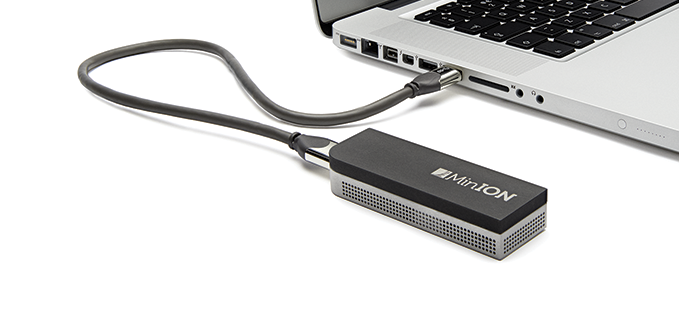
\includegraphics[width=1\textwidth]{imgs/minion.png}%
		\end{center}
	\end{figure}
\end{frame}


%%%%%%%%%%%%%%%%%%%%%%%%%%%%%%%%%%%%%%%%%%%%%%%%%%%%%%%%%%%%%%%%%%%%%%%%%%%%%%%%%%%%%%%
%% FRAME
\begin{frame}[fragile]{Technology}
	\begin{figure}
		\begin{center}
			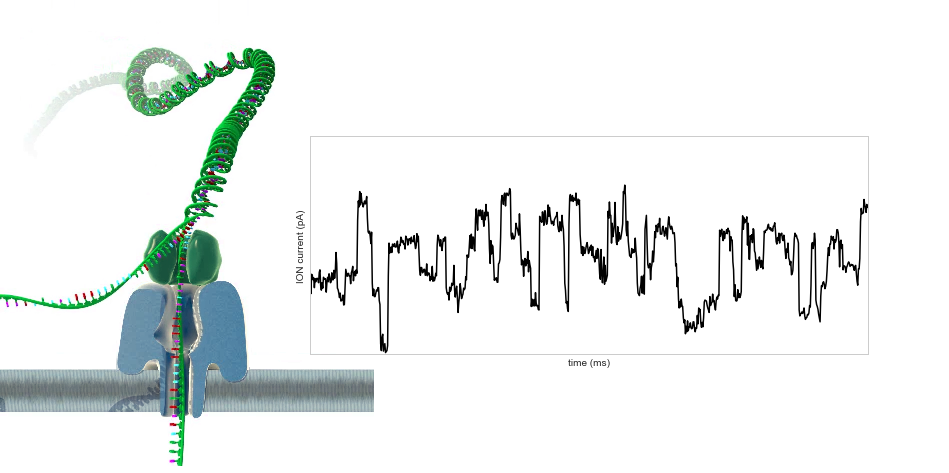
\includegraphics[width=1\textwidth]{imgs/nanopore_no_bases.png}%
		\end{center}
	\end{figure}
\end{frame}

%%%%%%%%%%%%%%%%%%%%%%%%%%%%%%%%%%%%%%%%%%%%%%%%%%%%%%%%%%%%%%%%%%%%%%%%%%%%%%%%%%%%%%%
%% FRAME
\begin{frame}[fragile]{Basecalling}
	\begin{figure}
		\begin{center}
			\includegraphics<1>[width=0.7\textwidth]{./imgs/basecall/basecall1.png}%
			\includegraphics<2>[width=0.7\textwidth]{./imgs/basecall/basecall2.png}%			
			\includegraphics<3>[width=0.7\textwidth]{./imgs/basecall/basecall3.png}%	
		\end{center}
	\end{figure}
\end{frame}

%%%%%%%%%%%%%%%%%%%%%%%%%%%%%%%%%%%%%%%%%%%%%%%%%%%%%%%%%%%%%%%%%%%%%%%%%%%%%%%%%%%%%%%
%% FRAME
\begin{frame}[fragile]{Basecalling options}

\alert{Metrichor}
\begin{itemize}
	\item only basecaller for ONT data
	\item proprietary software
	\item available as a cloud service
\end{itemize}

\alert{Goals}
\begin{itemize}
	\item local basecalling
	\item open-source
	\item speed, accuracy
\end{itemize}

\end{frame}


%%%%%%%%%%%%%%%%%%%%%%%%%%%%%%%%%%%%%%%%%%%%%%%%%%%%%%%%%%%%%%%%%%%%%%%%%%%%%%%%%%%%%%%
%% FRAME
\begin{frame}[fragile]{Existing solutions}
	\begin{itemize}
		\item Third-party: \textit{DeepNano, NanoCall}
		\item Official: \textit{MinKNOW, Nanonet, Albacore, Scrappie}
	\end{itemize}
	\alert{Idea?}
	\begin{itemize}
	\item Signal segmentation – event detection
	\item RNN, HMM (older version of \textit{Metrichor} and \textit{NanoCall})
	\end{itemize}
	
	
	\begin{figure}
		\begin{center}
			\includegraphics<1>[width=0.7\textwidth]{./imgs/segment/segmented_0.png}%
			\includegraphics<2>[width=0.7\textwidth]{./imgs/segment/segmented_1.png}%			
			\includegraphics<3>[width=0.7\textwidth]{./imgs/segment/segmented_2.png}%	
			\includegraphics<4>[width=0.7\textwidth]{./imgs/segment/segmented_3.png}%			
			\includegraphics<5>[width=0.7\textwidth]{./imgs/segment/segmented_4.png}%	
			\includegraphics<6>[width=0.7\textwidth]{./imgs/segment/segmented_5.png}%
			\includegraphics<7>[width=0.7\textwidth]{./imgs/segment/segmented_full.png}%				
		\end{center}
	\end{figure}
\end{frame}


%%%%%%%%%%%%%%%%%%%%%%%%%%%%%%%%%%%%%%%%%%%%%%%%%%%%%%%%%%%%%%%%%%%%%%%%%%%%%%%%%%%%%%%
%% FRAME
\begin{frame}[fragile]{Proposed solution}
	 end2end, CNN, CTC loss\\
	 speed, paralelization, sequental, eliminate shit \\
	 
	 variable length loss function
\end{frame}

%%%%%%%%%%%%%%%%%%%%%%%%%%%%%%%%%%%%%%%%%%%%%%%%%%%%%%%%%%%%%%%%%%%%%%%%%%%%%%%%%%%%%%%
%% FRAME
\begin{frame}[fragile]{CTC loss}
	\alert{Idea}: decode sequence from fixed-width output (softmax over alphabet)
	\begin{figure}
		\caption{Path "AAC-T"}
		\begin{center}
			\includegraphics<1>[width=0.7\textwidth]{./imgs/ctc/graph_0.png}%
			\includegraphics<2->[width=0.7\textwidth]{./imgs/ctc/graph_1.png}%	
		\end{center}
	\end{figure}
	\onslide<3->{
		\begin{equation}
		\begin{gathered}
			P(\pi | X) = \prod_{t=1}^{m} s_t(\pi_t)
		\end{gathered}
		\end{equation}
	}
	

\end{frame}

%%%%%%%%%%%%%%%%%%%%%%%%%%%%%%%%%%%%%%%%%%%%%%%%%%%%%%%%%%%%%%%%%%%%%%%%%%%%%%%%%%%%%%%
%% FRAME
\begin{frame}[fragile]{CTC loss}
	\alert{Idea}: decode sequence from fixed-width output
	\onslide<1->{
		\begin{equation}
			\begin{gathered}
			\label{eq:multiple}
			ACT = \begin{cases}
			decode(A, A, A, C, T) \\
			decode(A, A, C, -, T) \\
			decode(-, A, C, T, T)  \\
			decode(-, -, A, C, T)  \\
			decode(A, C, C, C, T)  \\
			\vdots \\
			decode(A, C, T, -, -) 
			\end{cases}
			\end{gathered}
		\end{equation}
	}
	\onslide<2->{	
		\begin{equation}
			\begin{gathered}
			P(Y | X) = \sum_{\pi \in decode^{-1}(Y)}^{} P(\pi | X)
			\end{gathered}
		\end{equation}
	}
\end{frame}

%%%%%%%%%%%%%%%%%%%%%%%%%%%%%%%%%%%%%%%%%%%%%%%%%%%%%%%%%%%%%%%%%%%%%%%%%%%%%%%%%%%%%%%
%% FRAME
\begin{frame}[fragile]{CTC loss}

Given the dataset $D = \{(X_i, Y_i)\}$, training objective is the maximization of the likelihood of each training sample  which is the same as the minimization of negative log likelihood:

	\begin{equation}
		\begin{gathered}
		L(D) = - \sum_{(X,Y)\in D}^{} ln P(Y | X)
		\end{gathered}
	\end{equation}
\end{frame}

%%%%%%%%%%%%%%%%%%%%%%%%%%%%%%%%%%%%%%%%%%%%%%%%%%%%%%%%%%%%%%%%%%%%%%%%%%%%%%%%%%%%%%%
%% FRAME
\begin{frame}[fragile]{Training}
		
	\begin{figure}
		\begin{center}
			\includegraphics<1>[width=1\textwidth]{./imgs/train/t1.png}%
			\includegraphics<2>[width=1\textwidth]{./imgs/train/t2.png}%
			\includegraphics<3>[width=1\textwidth]{./imgs/train/t3.png}%
			\includegraphics<4>[width=1\textwidth]{./imgs/train/t4.png}%
			\includegraphics<5>[width=1\textwidth]{./imgs/train/t5.png}%
		\end{center}
	\end{figure}
\end{frame}


%%%%%%%%%%%%%%%%%%%%%%%%%%%%%%%%%%%%%%%%%%%%%%%%%%%%%%%%%%%%%%%%%%%%%%%%%%%%%%%%%%%%%%%
%% FRAME
\begin{frame}[fragile]{Model}
	\begin{itemize}
		\item Residual CNN, 72 blocks, 2M parameters
		\item Maxpool every 24 blocks, reduction of dimensionality by factor 8
	\end{itemize}
	\begin{figure}
		\caption{Residual block}
		\begin{center}
			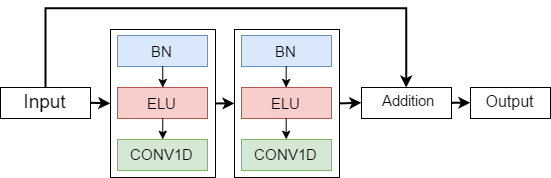
\includegraphics[width=0.7\textwidth]{./imgs/model/block_small.png}%

		\end{center}
	\end{figure}
\end{frame}



%%%%%%%%%%%%%%%%%%%%%%%%%%%%%%%%%%%%%%%%%%%%%%%%%%%%%%%%%%%%%%%%%%%%%%%%%%%%%%%%%%%%%%%
%% FRAME
\begin{frame}[fragile]{Results}
	\begin{itemize}
		\item Residual CNN, 72 blocks, 2M parameters
		\item Maxpool every 24 blocks, reduction of dimensionality by factor 8
	\end{itemize}
	\begin{figure}
		\caption{Residual block}
		\begin{center}
			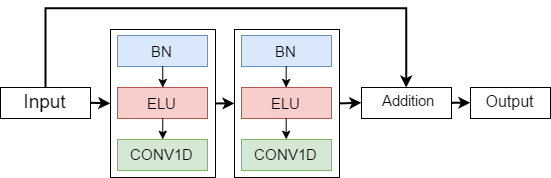
\includegraphics[width=0.7\textwidth]{./imgs/model/block_small.png}%
			
		\end{center}
	\end{figure}
\end{frame}

%%%%%%%%%%%%%%%%%%%%%%%%%%%%%%%%%%%%%%%%%%%%%%%%%%%%%%%%%%%%%%%%%%%%%%%%%%%%%%%%%%%%%%%
%% FRAME
\begin{frame}[fragile]{Future work}
	\begin{itemize}
		\item<1-> Scaled Exponential Linear Units (SELU), Jun 2017
		\item<3-> Facebook AI Research (FAIR) team: \textit{Convolutional Sequence to Sequence Learning}, May 2017
		\item<4-> ...
	\end{itemize}
	
	\onslide<2> {
		\begin{figure}
			\caption{Implementation}
			\begin{center}
				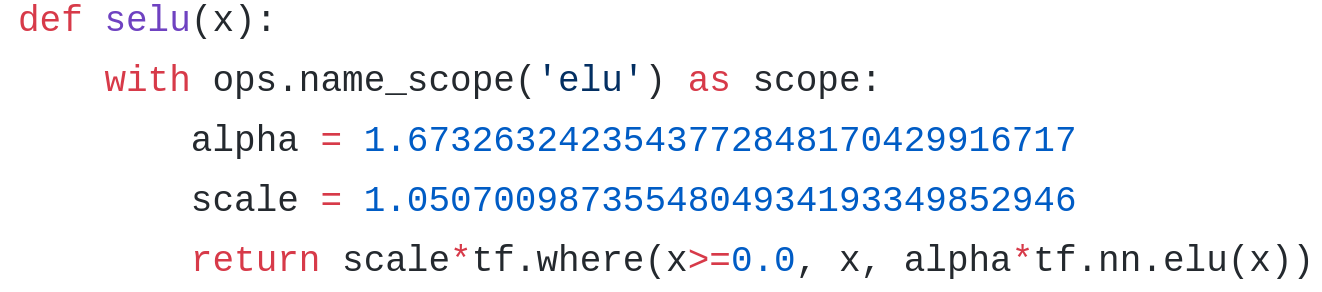
\includegraphics[width=0.7\textwidth]{./imgs/selu_tf.png}%
				
			\end{center}
		\end{figure}
	}
\end{frame}

%%%%%%%%%%%%%%%%%%%%%%%%%%%%%%%%%%%%%%%%%%%%%%%%%%%%%%%%%%%%%%%%%%%%%%%%%%%%%%%%%%%%%%%
%% FRAME
\begin{frame}[fragile]{End}
	\vfill
	\begin{center}  
		Thank you for your attention!
	\end{center}
	
	\uncover<2->{ 
		\begin{center}  \large Any questions? \end{center} 
	} 
	\vfill
\end{frame}
\end{document}
